\documentclass[12pt,fleqn]{article}
\usepackage{vkCourseML}
\hypersetup{unicode=true}
%\usepackage[a4paper]{geometry}
\usepackage{breakurl}
\usepackage{wrapfig}
\usepackage{subcaption}
\usepackage{graphicx}
\usepackage{cite}
\interfootnotelinepenalty=10000

\newcommand{\subtitle}[1]{
  \posttitle{
    \par\end{center}
    \begin{center}\large#1\end{center}
    \vskip0.5em}
}

\newcommand{\R}{\mathbb{R}}

\begin{document}
\title{Анализ временных рядов методами DL}
\author{Введение в эффективные системы ML\\Спецкурс ММП ВМК МГУ\\Алексеев Илья, @voorhs}
\date{18 окт 2024}
\maketitle

\section{Введение}

\subsection{Что такое временные ряды}

Одномерным временным рядом (univariate time series) мы будем называть числовую последовательность $x_1,\ldots,x_T$. Число $x_t\in\R$ мы называем наблюдением, или замером, (observation) в момент времени $t$ (timestamp). Эти названия отражают, в каких областях обычно возникают временные ряды: замер температуры воздуха, концентрации вещества и проч.

Многомерным временным рядом (multivariate time series) мы будем называть последовательность векторов $x_1,\ldots,x_T$. В данном случае наблюдением будет целый вектор $x_t\in\R^C$. Он представляет собой замеры сразу нескольких величин. Например, вместе с температурой можно мерить давление и влажность воздуха. Отличие $C$-мерного временного ряда от набора из $C$ одномерных временных рядов в том, что в многомерном ряде обычно предполагают, что компоненты вектора $x_t$ относятся к одному моменту времени.

\subsection{Задачи анализа временных рядов}

\begin{figure}[!htb]
    \centering
    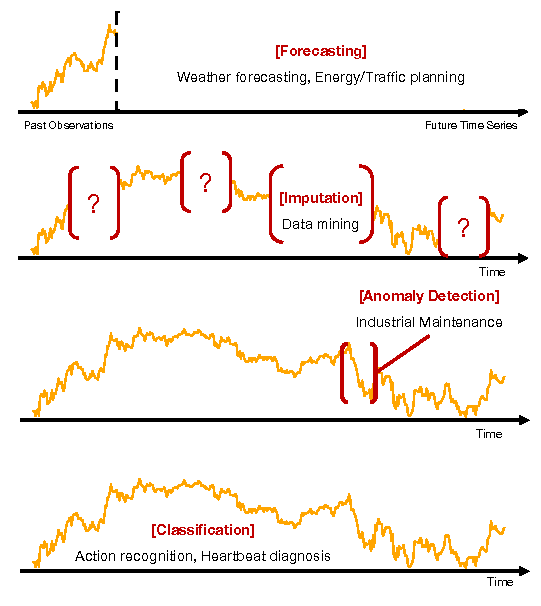
\includegraphics[width=0.5\linewidth]{LaTeX/images/tasks.pdf}
    \caption{Задачи анализа временных рядов.}
    \label{fig:tasks}
\end{figure}

Прогнозирование (forecasting) временного ряда заключается в предсказании неизвестных будущих значений временного ряда на основе известных исторических значений. Обычно разделяют на два подтипа: краткосрочное (short-term) и долгосрочное прогнозирование (long-term forecasting). Эти задачи отличаются не временными промежутками (часы, дни, месяцы, годы), а количеством наблюдений (десятки, сотни, тысячи), которое требуется предсказать. Такое разделение объясняется двумя причинами. В первую очередь — тем, что модель, дающая на выходе тысячи векторов должна быть вычислительно эффективной. Во вторую очередь — тем, что не все методы способны промоделировать зависимости между тысячами векторов.

Классификация временных рядов заключается в присвоении метки всему ряду. Самая популярный пример задачи — это классификация ЭКГ на нормальные и патологические.

Обнаружение аномалий (anomaly detection) состоит в выявлении атипичных значений или сегментов временного ряда. Чаще всего встречается для выявления сбоев в работе оборудования по замерам с датчиков.

Заполнение пропусков (imputation) — это восстановление пропущенных значений.

\section{Нейросетевые методы для работы с временными рядами}

Для анализа временных рядов можно применять любые нейросети, работающие с последовательностями: CNN, RNN, Transformer. Если длина временного ряда никогда не меняется, можно применять даже MLP. 

\subsection{Применение полносвязных сетей}

\begin{itemize}
    \item для классификации можно построить сеть, сужающуюся до слоя шириной в число классов
    \item для прогнозирования можно
    \begin{itemize}
        \item построить сеть, сужающуюся до слоя шириной в число прогнозируемых значений \cite{ltsflinear}
        \item а можно использовать авто-регрессионное прогнозирование
    \end{itemize}
    \item можно применять современные MLP-based архитектуры вроде MLP-mixer, FNet, gMLP \cite{tsmixer}
\end{itemize}

\begin{figure}[!htb]
    \centering
    \begin{minipage}{0.45\linewidth}
        \centering
        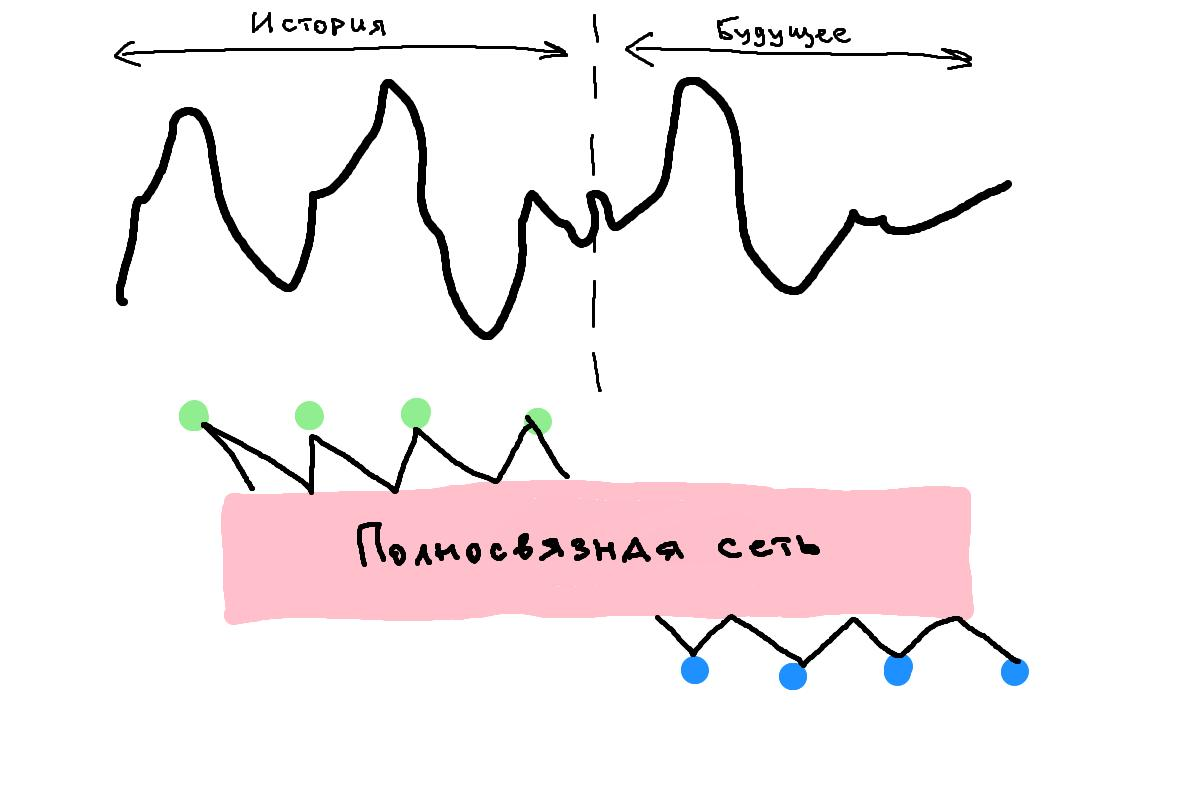
\includegraphics[width=\linewidth]{illustrations/mlp-forecasting.jpg}
        \caption{MLP forecasting}
        \label{fig:mlp-forecasting}
    \end{minipage}
    \begin{minipage}{0.45\linewidth}
        \centering
        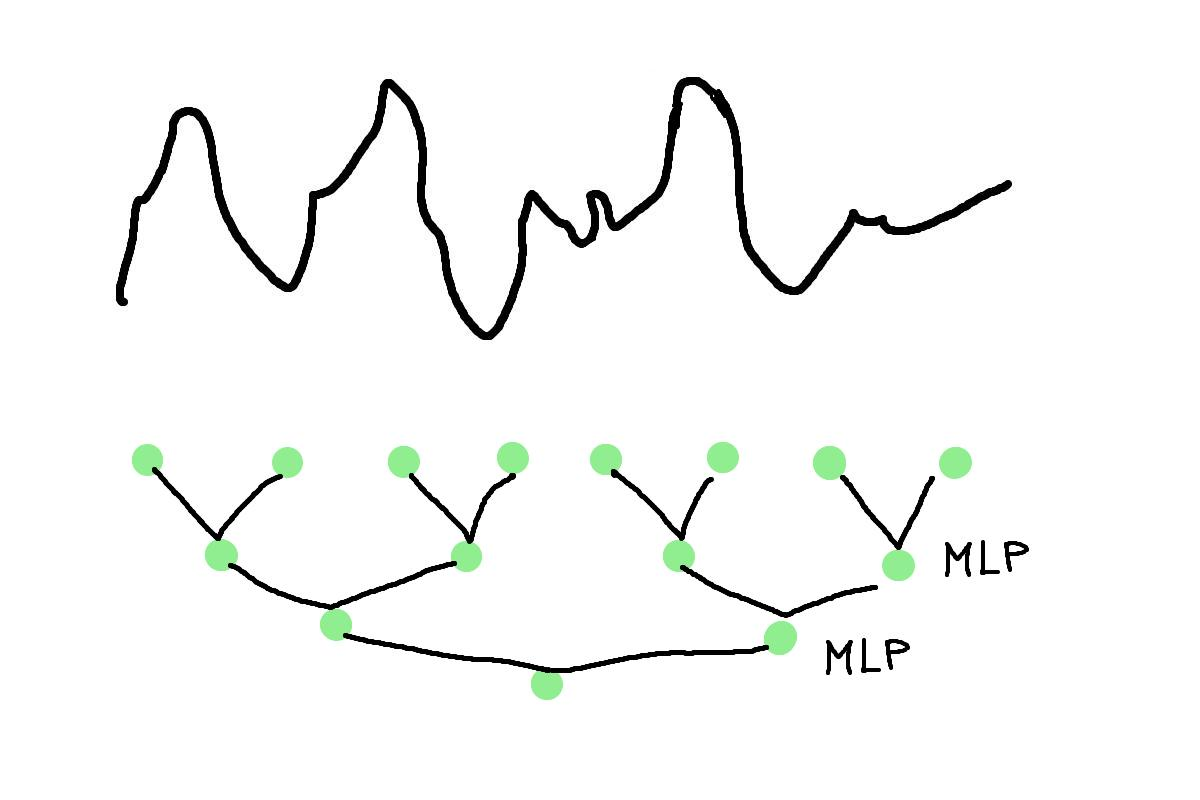
\includegraphics[width=\linewidth]{illustrations/mlp-clf.jpg}
        \caption{MLP classification}
        \label{fig:mlp-classification}
    \end{minipage}
\end{figure}


\subsection{Применение свёрточных сетей}

\begin{itemize}
    \item для классификации можно построить сеть, сужающуюся до слоя шириной в число классов \cite{inception}
    \item для прогнозирования можно
    \begin{itemize}
        \item построить сеть, сужающуюся до слоя шириной в число прогнозируемых значений
        \item либо использовать казуальные свёртки в авторегрессионном режиме \cite{tcnpaper, wavenet, moderntcn}
    \end{itemize}
\end{itemize}

\begin{figure}[!htb]
    \centering
    \begin{minipage}{0.45\linewidth}
        \centering
        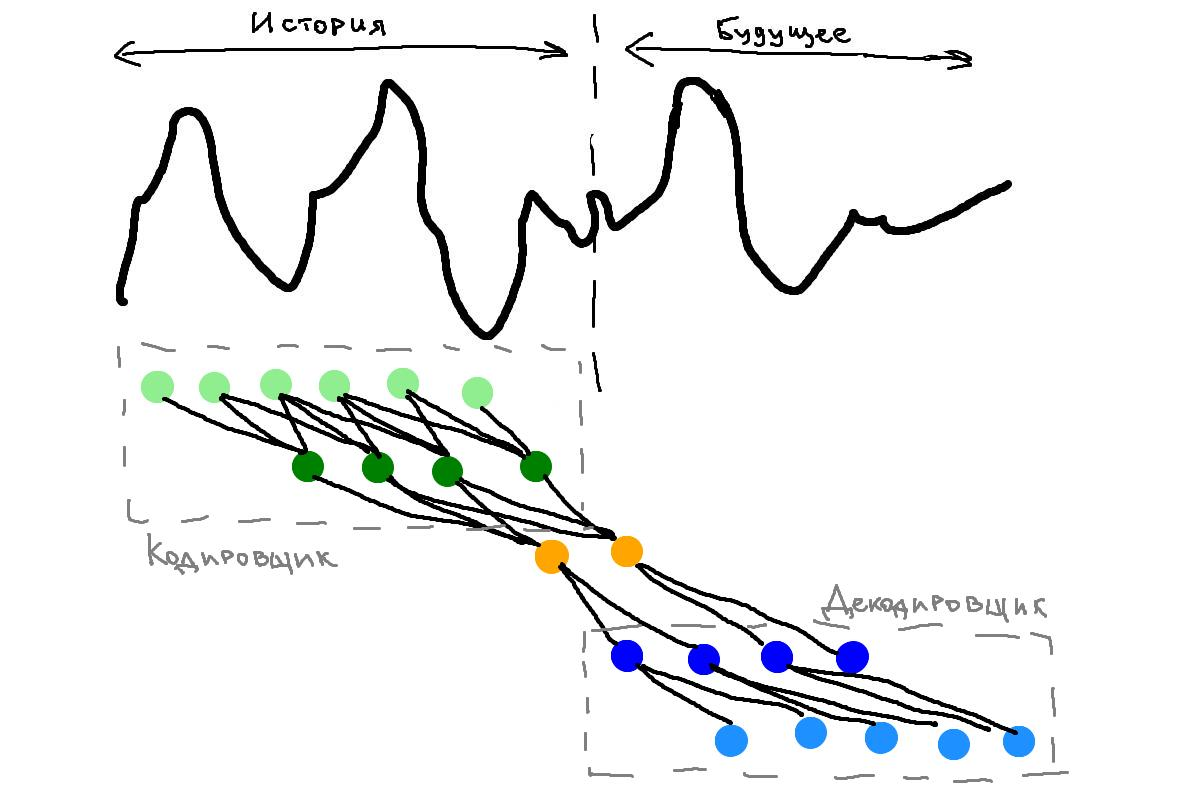
\includegraphics[width=\linewidth]{illustrations/cnn-forecasting.jpg}
        \caption{CNN forecasting}
        \label{fig:mlp-forecasting}
    \end{minipage}
    \begin{minipage}{0.45\linewidth}
        \centering
        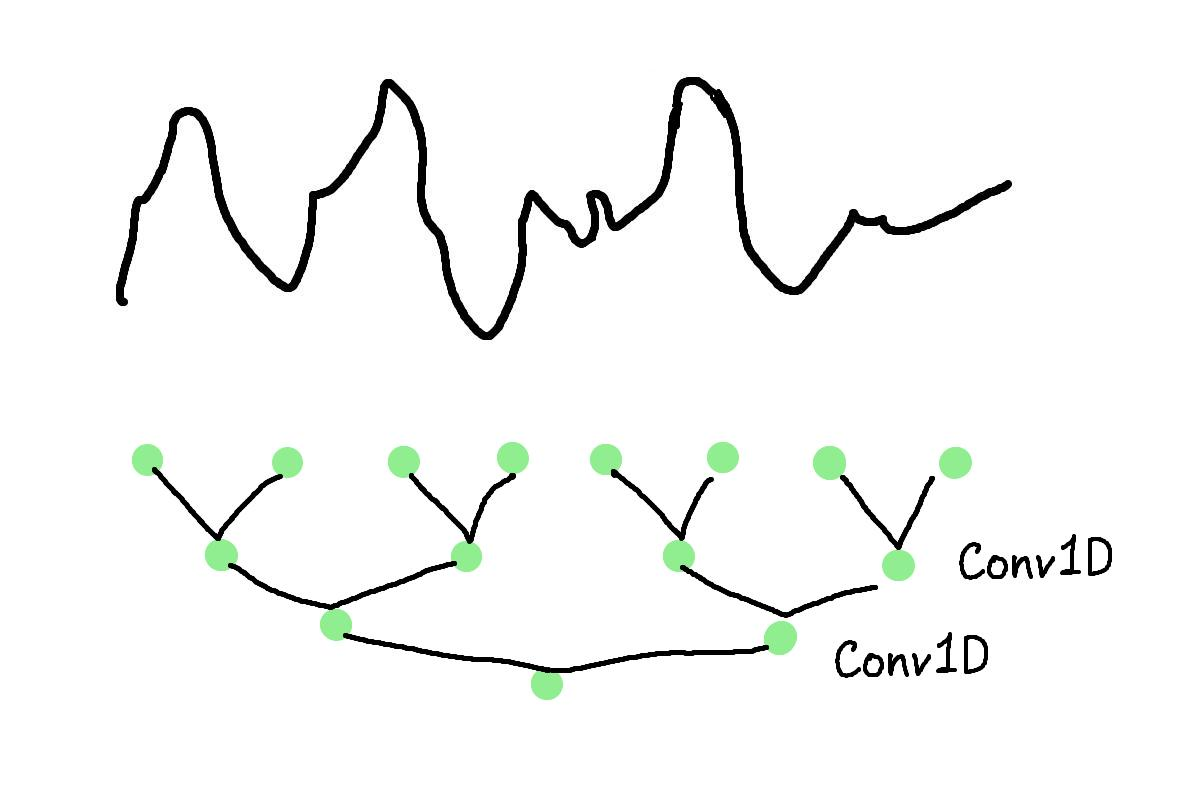
\includegraphics[width=\linewidth]{illustrations/cnn-clf.jpg}
        \caption{CNN classification}
        \label{fig:mlp-classification}
    \end{minipage}
\end{figure}

\subsection{Применение рекуррентных сетей}

\begin{itemize}
    \item для классификации можно
    \begin{itemize}
        \item построить обычную сеть (даже двунаправленную) и взять выходное представление с последнего момента времени,
        \item либо построить сужающуюся сеть (что в целом для RNN экзотика, но возможно)
    \end{itemize}
    \item для предсказания можно использовать обычную казуальную архитектуру \cite{deepar}

\end{itemize}

\begin{figure}[!htb]
    \centering
    \begin{minipage}{0.45\linewidth}
        \centering
        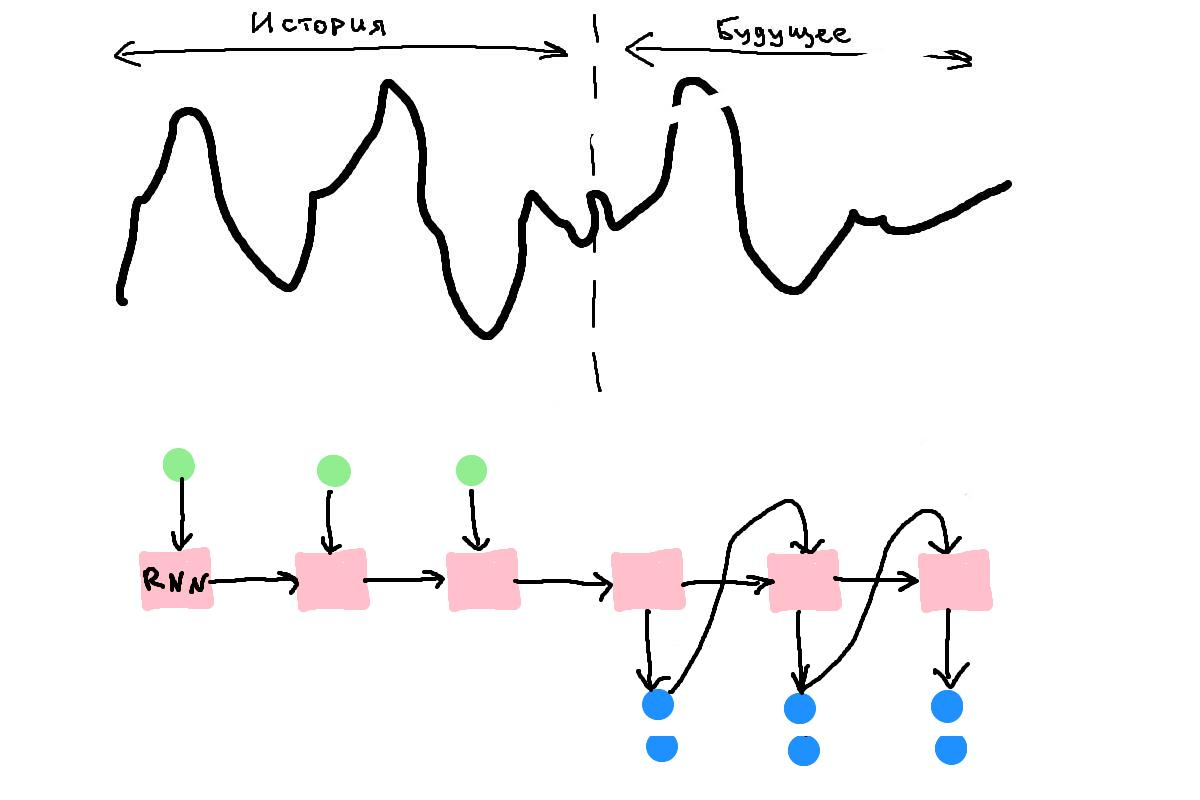
\includegraphics[width=\linewidth]{illustrations/rnn-forecasting.jpg}
        \caption{RNN forecasting}
        \label{fig:mlp-forecasting}
    \end{minipage}
    \begin{minipage}{0.45\linewidth}
        \centering
        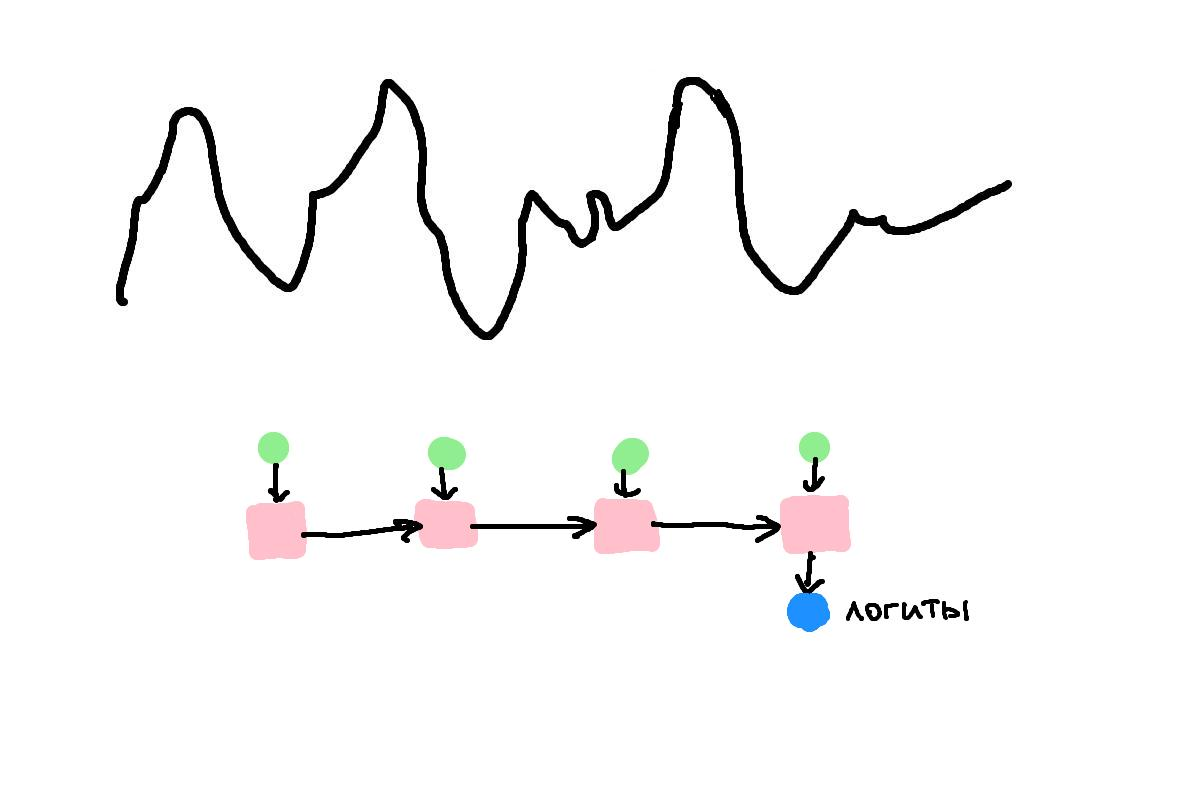
\includegraphics[width=\linewidth]{illustrations/rnn-clf-1.jpg}
        \caption{RNN classification}
        \label{fig:mlp-classification}
    \end{minipage}\\
    \begin{minipage}{0.45\linewidth}
        \centering
        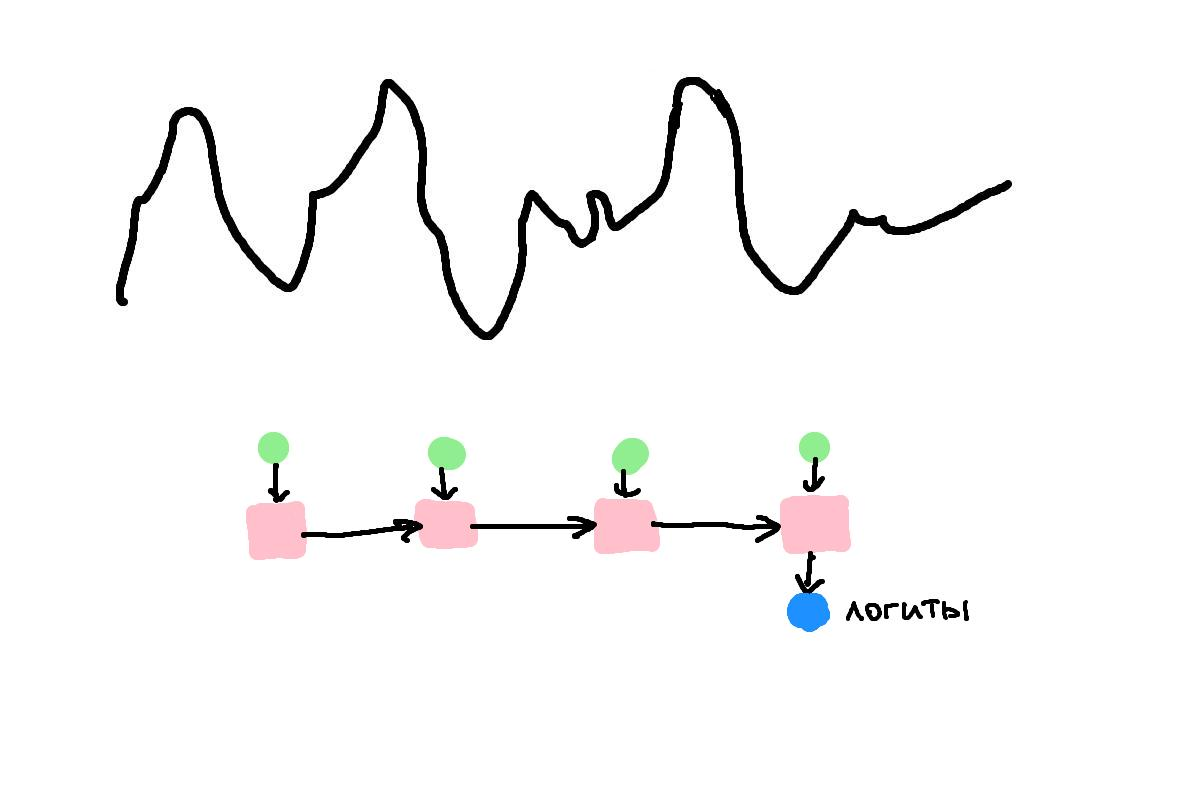
\includegraphics[width=\linewidth]{illustrations/rnn-clf-1.jpg}
        \caption{RNN classification}
        \label{fig:mlp-classification}
    \end{minipage}
\end{figure}

Есть еще экзотические и передовые технологии SSM \cite{ssm}. Если вкратце, то это RNN вычисляющая коэффициенты оптимальной аппроксимации исторических данных с помощью линейной комбинации системы полиномов Лагранжа или Лежандра. Этот материал не является предметом настоящего занятия.

\subsection{Применение трансформеров}

\begin{itemize}
    \item для классификации можно использовать двунаправленный трансформер и агрегировать представления с последнего слоя
    \item для предсказания можно
    \begin{itemize}
        \item использовать трансформер в казуальном режиме,
        \item но чаще всего берут энкодер-декодер \cite{informer, nst}. В декодере не используют авторегрессионное предсказание, вместо этого (поскольку известна длина выходной последовательности) используют плейсхолдеры, которые после прохода через каждый слой как бы заполняются новой информацией и формируют итоговое предсказание
    \end{itemize}
\end{itemize}


\begin{figure}[!htb]
    \centering
    \begin{minipage}{0.45\linewidth}
        \centering
        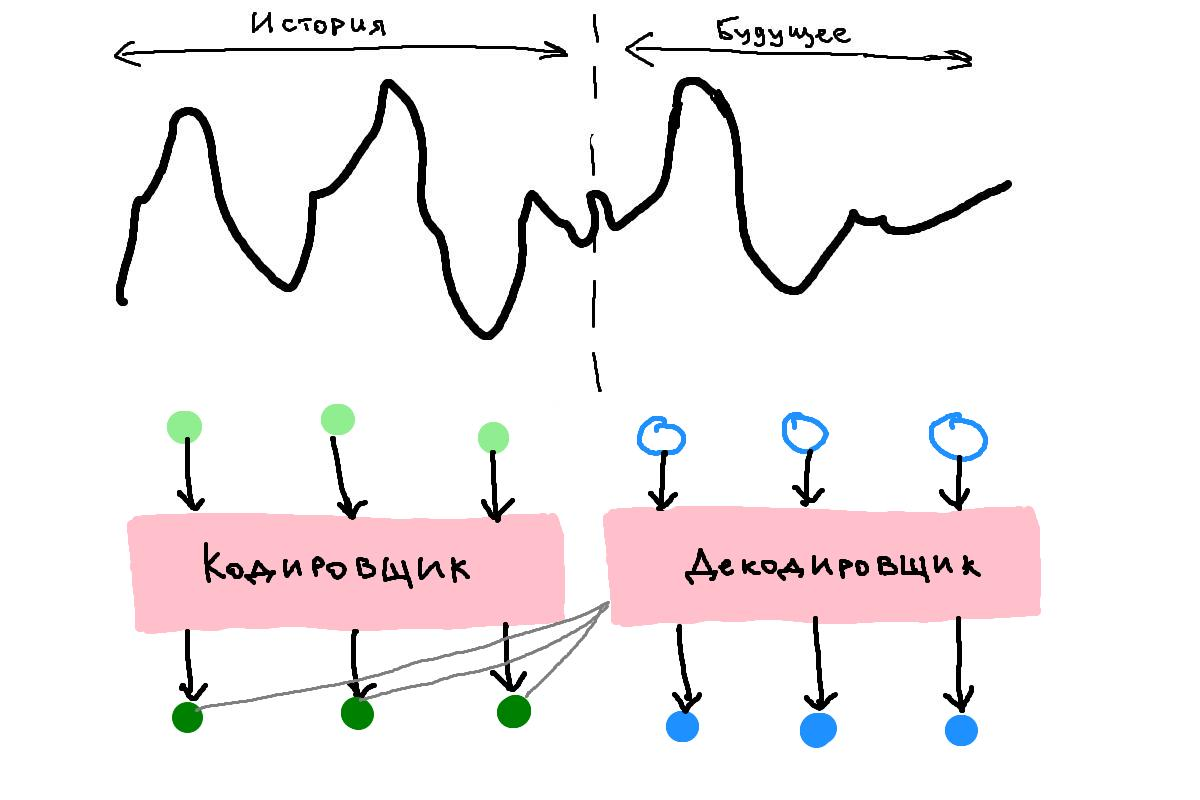
\includegraphics[width=\linewidth]{illustrations/transformer-forecasting.jpg}
        \caption{Transformer forecasting}
        \label{fig:mlp-forecasting}
    \end{minipage}
    \begin{minipage}{0.45\linewidth}
        \centering
        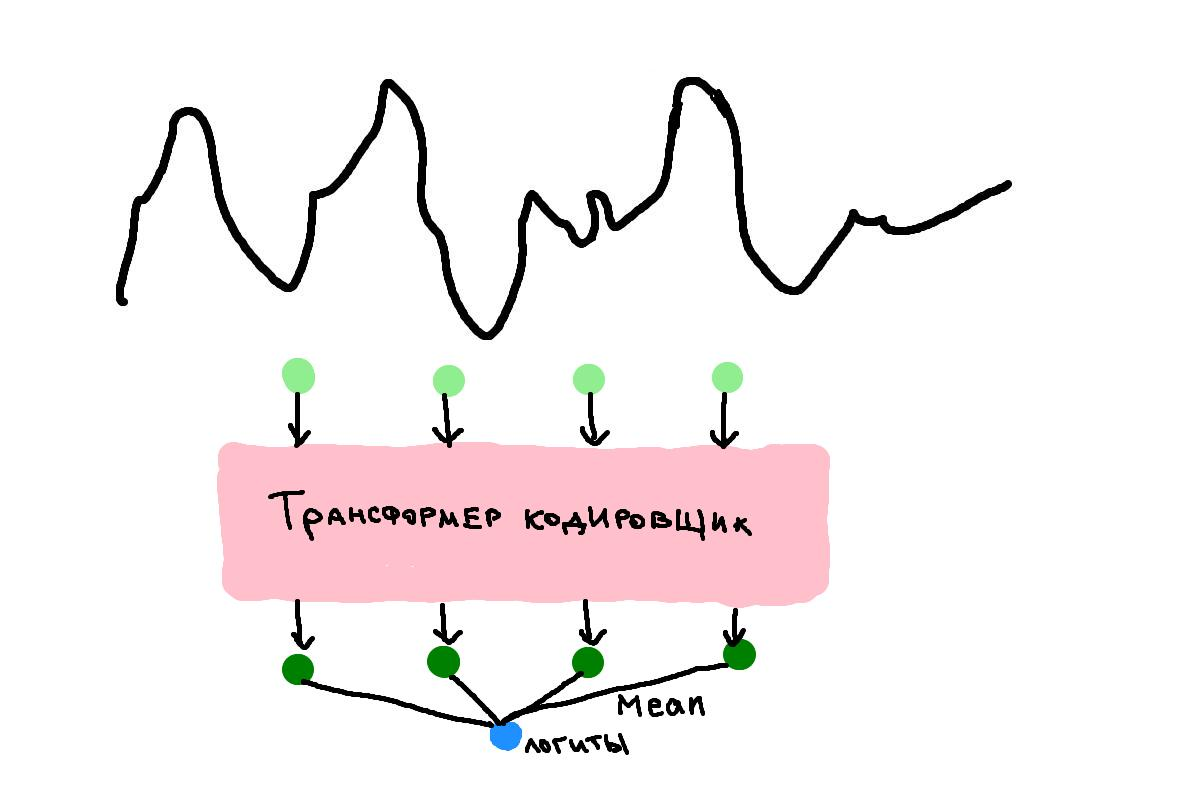
\includegraphics[width=\linewidth]{illustrations/transformer-clf.jpg}
        \caption{Transformer classification}
        \label{fig:mlp-classification}
    \end{minipage}
\end{figure}


Чаще всего признаки временного ряда не подаются в сыром виде в нейросеть. Помимо прочих препроцессингов, всегда используется проецирование с помощью одного или нескольких полносвязных слоев в большую размерность вроде 96 или 128. Такие представления заменяют эмбеддинги.

\section{Архитектуры}

\subsection{Работа с периодичными рядами. TimesNet}

Большинство временных рядов, встречающихся на практике, имеют периоды. Поэтому очень полезно уметь их выделять. Проще всего это сделать с помощью быстрого преобразования Фурье. Оно переводит функцию времени $f(t)$ в функцию частоты $F(\nu)$. Если пики функции $f(t)$ соответствуют мощности замера $t$, то пики функции $F(\nu)$ — степени присутствия частоты $\nu$.

Допустим, мы выделили одну из пиковых частот $\nu$. Мы можем порезать весь временной ряд на отрезки длины $T\nu$ и сопоставить их друг с другом. Тогда мы получим двумерное представление временного ряда в виде матрицы, где в столбцах находятся замеры из одного кусочка, а в строках точки — точки из разных кусочков, но с одинаковой фазой относительно периода $1/\nu$. Это представление обладает важным свойством: оно интерпретируемо как изображение. Действительно, "пиксели", соседние данному, должны быть очень похожи.

\begin{figure}[!htb]
    \centering
    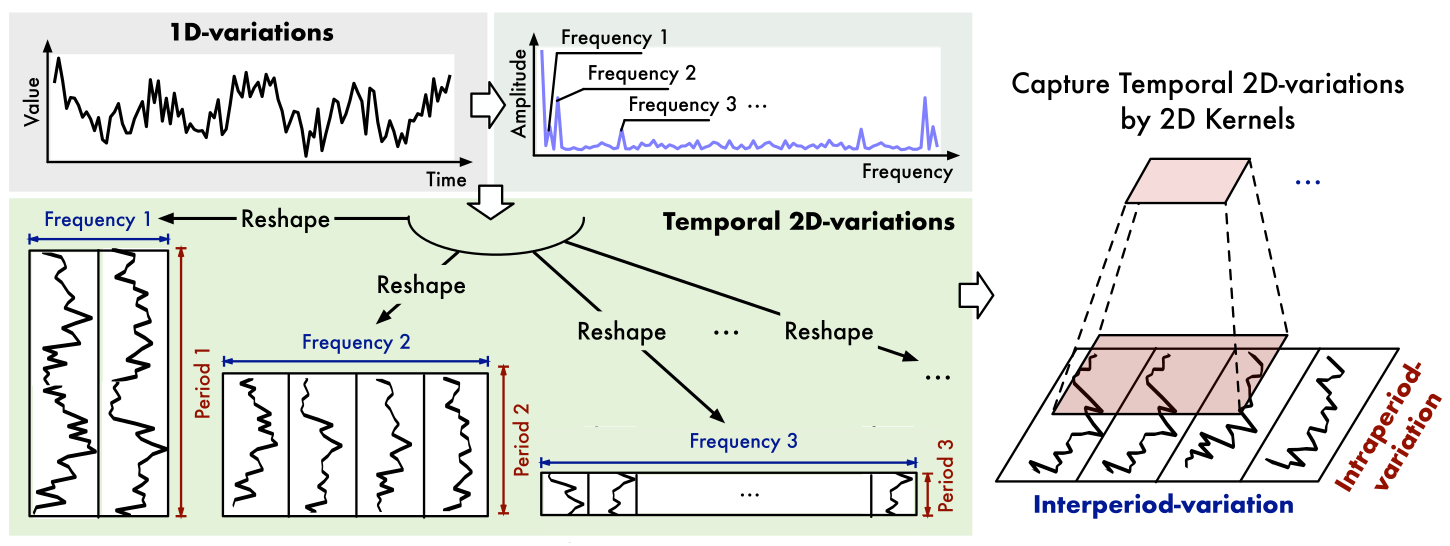
\includegraphics[width=0.5\linewidth]{notes.assets/image-20241018014918302.png}
    \caption{Фурье-анализ и получение двумерного представления временного ряда}
    \label{fig:2d-representation}
\end{figure}

Архитектура TimesNet \cite{timesnet} состоит из последовательности TimesBlock'ов, каждый из которых выделяет $k$ пиковых частот, формирует двумерные представления для каждой частоты и применяет к ним двумерную свёртку, как будто это изображения. Результирующие преобразования агрегируются и формируют выход TimesBlock'а. Такое разделение на $k$ представлений играет роль, схожую той, что головы играют в мультиголовочном аттеншене.

\begin{figure}[!htb]
    \centering
    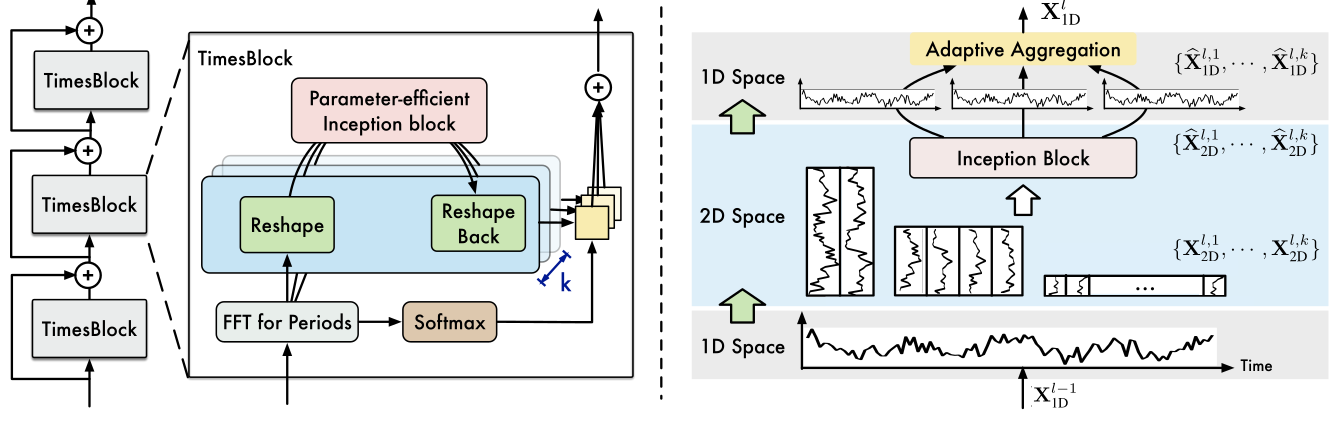
\includegraphics[width=0.5\linewidth]{notes.assets/image-20241018015234974.png}
    \caption{Архитектура TimesNet}
    \label{fig:timesnet}
\end{figure}

\subsection{Работа с нестационарными временными рядами}

Временной ряд называют стационарным, если со временем среднее и дисперсия его значений не меняются. Нестационарные ряды наиболее тяжелы для анализа методами DL. Это связано с известным фактом, что нейросети тяжело учатся, когда на вход подаются величины с постоянно меняющейся магнитудой. Особо осведомленные читатели знают, что причиной тому стохастическая оптимизация.

\begin{figure}[!htb]
    \centering
    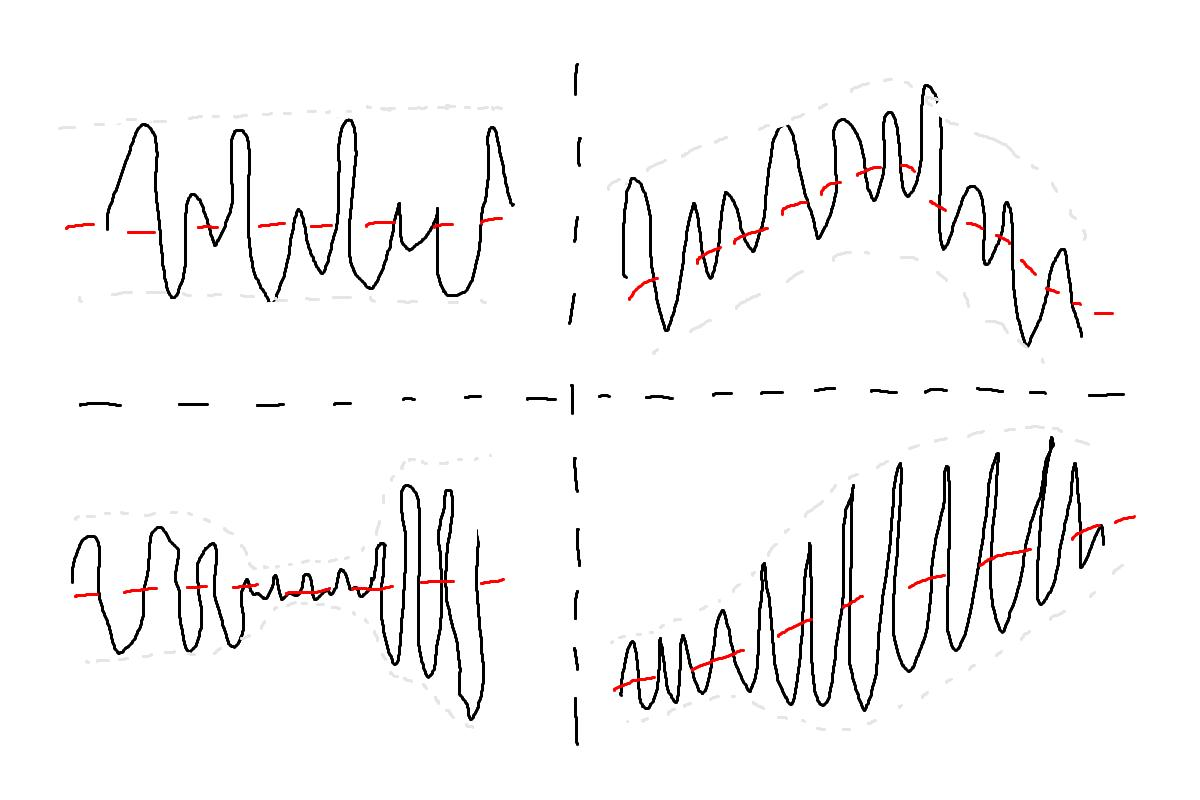
\includegraphics[width=0.5\linewidth]{illustrations/stationarity.jpg}
    \caption{Примеры нестационарных временных рядов}
    \label{fig:stationarity}
\end{figure}

Трендом временного ряда называют долгосрочное изменение. Другими словами, это наиболее общее направление, которое можно получить сглаживанием или усреднением с помощью скользящего окна. Тренд связан с понятием среднего. Если произвести преобразование временного ряда таким образом, чтобы тренд и дисперсия стали константными, то в данных останутся только мелкомасштабные изменения, которые гораздо проще моделировать. Такое преобразование называют стационаризацией временного ряда. На идее стационаризации основано большинство методов анализа временных рядов.

\subsubsection{Разложение на компоненты}

Трендово-циклической компонентной называют не наиболее общее направление временного ряда. Будем воспринимать это как элемент иерархии, находящийся на ступень ниже. Обычно цикличностью ряда называют его свойство повторять предыдущие значения. Это не совсем периодичность, поскольку эти повторения могут происходить с разной регулярностью.

Если убрать из данных трендово-циклическую компоненту, оставшуюся компоненту называют сезонной.

\textbf{Autoformer}

Введем операцию разложения на две компоненты, трендовую и сезонную:

\begin{align*}
x_\text{trend}&=\text{MovAvg}(\text{Padding}(x)),\\
x_\text{season}&=x-x_\text{trend}.
\end{align*}

Напомним, что операция moving average заключается во взятии бегущего среднего $k$ последовательных замеров. Нулевой падинг добавляется с краев, чтобы длина последовательности не менялась (стандартный прием).

Введенную операцию разложения можно применить внутри трансформера архитектуры энкодер-декодер. На вход кодировщику подается ненормированный ряд, внутри каждого трансформерного блока выделяется трендовая часть и отбрасывается. Это сделано, чтобы обрабатывать только сезонную часть. То есть с проходом через блоки кодировщика модель выделяет все более мелкомасштабные изменения.

Это отражает то, что основную информацию несут локальные зависимости, отделенные от общего тренда. Если энкодер обрабатывает сезонную компоненту прошлого, то свою очередь декодер будет предсказывать сезонную компоненту для будущего.

В autoformer \cite{autoformer} есть сразу два набора плейсхолдеров: для сезонной и трендовой компоненты. По мере прохождения через блоки кодировщика, эти компоненты как бы уточняются и наполняются информацией. Это отражает важность нестационарной информации для предсказания.

\begin{figure}[!htb]
    \centering
    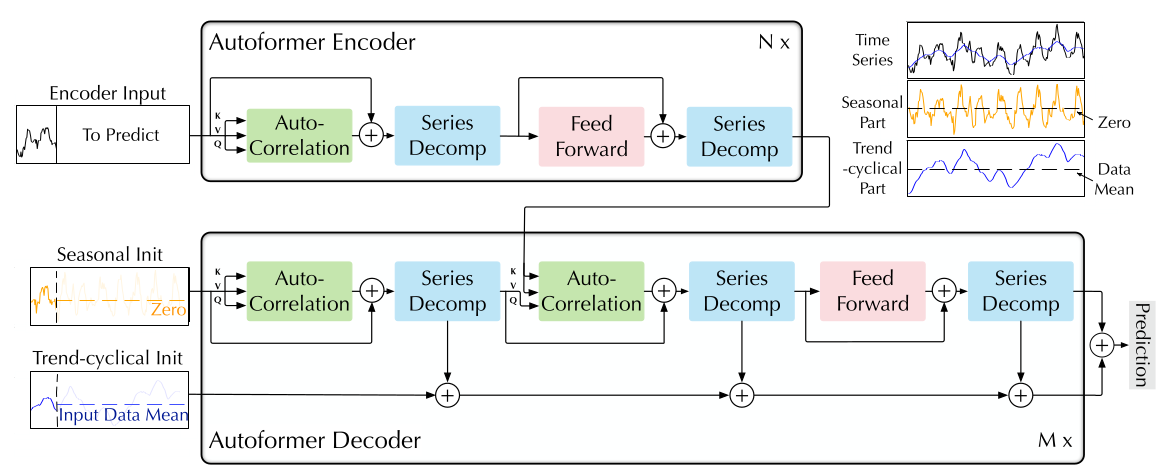
\includegraphics[width=0.5\linewidth]{notes.assets/image-20241018010712472.png}
    \caption{Как трендовая и сезонная компоненты используются в Autoformer}
    \label{fig:decomp}
\end{figure}

\textbf{AutoCorrelation}

Дополнительно в autoformer учитываются периоды, но более хитрым способом, нежели это было в TimesNet. Для случайного процесса можно определить функционал автокорреляции:
$$
\mathcal{R}_{xx}(\tau)=\lim_{L\to\infty}{1\over L}\sum_{t=1}^L x_tx_{t-\tau}.
$$
Этот функционал характеризует схожесть процесса $\{x_t\}$ с процессом $\{x_{t-\tau}\}$. Это может служить мерой уверенности, что процесс периодичен с длиной периода $\tau$. Для временных рядов (как реализаций случайного процесса) этот функционал тоже можно определить. Посчитать его можно с помощью FFT.

Если до этого периоды были головами в ансамбле, то теперь периоды служат токенами в механизме внимания:

\begin{align}
\tau_1,\ldots,\tau_k&=\arg\text{topk}\{\mathcal{R}_{Q,K}(\tau)\}\\
\alpha_1,\ldots,\alpha_k&=\text{Softmax}(\mathcal{R}_{Q,K}(\tau_1),\ldots,\mathcal{R}_{Q,K}(\tau_k))\\
\text{AutoCorrelation}(Q,K,V)&=\sum_{i=1}^k\alpha_i\text{Roll}(V,\tau_i).
\end{align}

Такая операция напрямую вытягивает похожие моменты из прошлого из формирует предсказание как взвешенное среднее между этими моментами. Операция $\text{Roll}(X,\tau)$ совершает циклический сдвиг во временном ряде так, чтобы сопоставить точки находящиеся в одной фазе относительно периода $\tau$.

\begin{figure}[!htb]
    \centering
    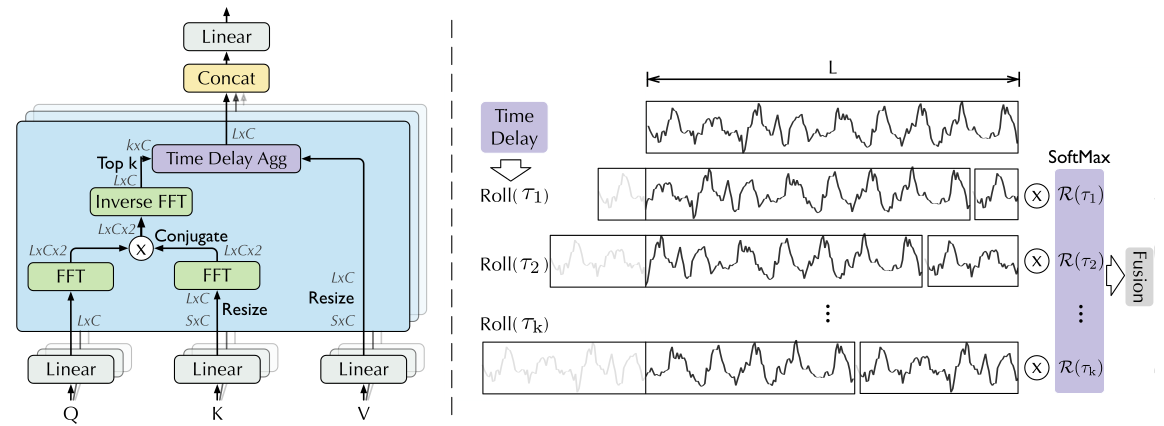
\includegraphics[width=0.5\linewidth]{notes.assets/image-20241018013325489.png}
    \caption{Механизм автокорреляции в Autoformer}
    \label{fig:autocorrelation}
\end{figure}

\subsubsection{Нормализация. RevIN}

Архитектура autoformer достаточно тяжеловесна для восприятия. Существует метод, который тоже борется с проблемой анализа нестационарных рядов, однако делает это куда более простым и изящным способом.

Известным примером является метод RevIN для прогнозирования \cite{revin}. Он заключается в следующем: что если нормализовать данные перед подачей в нейросеть, а на выходе произвести обратное преобразование и вернуть среднее и дисперсию. На входе используется instance нормализация с обучаемыми параметрами $\gamma,\delta$:
$$
\mu={1\over T}\sum_{t=1}^T x_t,\quad \sigma^2={1\over T}\sum_{t=1}^T(x_t-\mu)^2,\quad \widehat x_t=\gamma\circ{x_t-\mu\over\sqrt{\sigma^2+\varepsilon}}+\delta.
$$

Ряд $\widehat x\in\R^{T\times C}$ подается на вход нейросети, которая выдает предсказания $\widetilde y\in\R^{N\times C}$ для будущих $N$ замеров. К ним применяется обратное преобразование:
$$
y_t=\sqrt{\sigma^2+\varepsilon}\circ{\tilde y_t-\delta\over\gamma}+\mu.
$$
Название метода расшифровывается как reversible instance normalization. Во-первых, это не совсем стационаризация, скорее просто нормализация. Но нормализация для нейросетей играет большую роль. Во-вторых, это не нормализация всей обучающей выборки по каждому признаку, а это нормализация только внутри одного временного ряда. То есть instance нормализация может преобразовать два ряда с совершенно разными средними и дисперсиями в одинаковый. И в этом состоит предположение о том, что намного важнее предсказывать какие-то локальные динамики, чем учитывать, что <<этот ряд в диапазоне [5,10], а этот ряд в диапазоне [100,300]>>. Если между этими рядами есть что-то общее, то нейросеть не увидит этого из-за огромной разницы в масштабах.

\subsubsection{Нормализация. Non-Stationary Transformer}

На самом деле информация о среднем и дисперсии тоже ценна. Она может сообщать о природе ряда. Идея Non-Stationary Transformer (будем называть NST \cite{nst}) в том, чтобы учесть эту информацию не только на входе и выходе модели, но и внутри.

Итак, NST вооружен обратимой нормализацией, как и RevIN. Правда авторы NST обошлись без обучаемых параметров:
$$
\widehat x_t={x_t-\mu\over\sqrt{\sigma^2+\varepsilon}},\quad y_t=\sqrt{\sigma^2+\varepsilon}\circ \tilde y_t+\mu.
$$
Нормализованный ряд $\widehat x\in\R^{T\times C}$ не содержит информации о среднем и дисперсии. Он подается на вход сначала полносвязным слоям, играющим роль эмбедера, а затем скармливается трансформеру. Как использовать информацию об изначальном ненормализованном ряде внутри трансформера? Самое важное место в трансформере — это блоки с аттеншеном. Попытаемся проанализировать, как отличается аттеншен с пре-нормализацией и без ней. Чтобы упростить анализ, сделаем предположение, что в нейросети нет функций активаций и прочих нелинейностей, кроме операции аттеншена. Результат анализа, полученный при таком предположении мы потом попытаемся применить к общему нелинейному случаю.

\textbf{Линейный случай}

Механизм внимания:
$$
\text{Attn}(Q,K,V)=\text{Softmax}\left({QK^T\over\sqrt{d_k}}\right)V.
$$
Представления $Q,K,V$ являются результатами линейного преобразования входа $x$ (согласно нашему предположению), т.е. $Q=f_Q(x)$, $K=f_K(x)$, $V=f_V(x)$. Обозначим $Q'=f_Q(\widehat x)$, $K'=f_K(\widehat x)$, $V'=f_V(\widehat x)$.

Как отличаются $Q'$ от $Q$?
$$
Q'=f_Q\left({x-\textbf{1}\mu^T\over\sigma}\right)={f_Q(x)-\textbf{1}f_Q(\mu)^T\over\sigma}={Q-\textbf{1}\mu_Q^T\over\sigma},\quad\mu_Q={1\over T}\sum_{t=1}^Tq_t.
$$
По аналогии будет
$$
K'={K-\textbf{1}\mu_K^T\over\sigma}.
$$
Как отличаются $Q'K'^T$ от  $QK^T$?
$$
Q'K'^T={1\over\sigma^2}(QK^T-\textbf{1}(\mu_Q^TK^T)-(Q\mu_K)\textbf{1}^T+\textbf{1}(\mu_Q^T\mu_K)\textbf{1}^T).
$$
Как отличается $\text{Attn}(Q',K',V')$ от $\text{Attn}(Q,K,V)$? Выражение $QK^T$ входит в аттеншен под софтмаксом. Софтмакс не меняется, если ко всем компонентам прибавить одно и то же число:
\begin{align*}
\text{Softmax}\left({QK^T\over\sqrt{d_k}}\right)&=\text{Softmax}\left({\sigma^2Q'K'^T+\textbf{1}(\mu_Q^TK^T)+(Q\mu_K)\textbf{1}^T-\textbf{1}(\mu_Q^T\mu_K)\textbf{1}^T\over\sqrt{d_k}}\right)\\
&=\text{Softmax}\left({\sigma^2Q'K'^T+\textbf{1}(\mu_Q^TK^T)\over\sqrt{d_k}}\right)    
\end{align*}

Получили, что подавая на вход трансформеру (полностью линейному) нормализованный временной ряд, мы имеем возможность прямо внутри трансформера посчитать аттеншен для ненормализованного временного ряда. Тем самым мы учтем среднее и дисперсию исходных данных.

Проанализируем полученное выражение. Что именно привносит информацию о распределении? Число $\sigma^2$ и $K^T\mu_Q$ — это статистики, посчитанные на исходном временном ряде.

\textbf{Общий случай}

Но в общем случае мы не можем использовать полностью линейный трансформер. А значит использовать $\sigma^2$ становится неосмысленно, а доступа к $K\mu_Q$ у нас по просту нет.

Основная идея de-stationary attention состоит в том, чтобы аппроксимировать $\tau\approx\sigma^2$ и $\Delta\approx K\mu_Q$ как некоторые функции от исходного ряда:
$$
\log\tau=\text{MLP}(\sigma,x),\quad\Delta=\text{MLP}(\mu,x),\\
\text{Attn}(Q',K',V')=\text{Softmax}\left({\tau Q'K'^T+\textbf{1}\Delta^T\over\sqrt{d_k}}\right)V'.
$$

\begin{figure}[!htb]
    \centering
    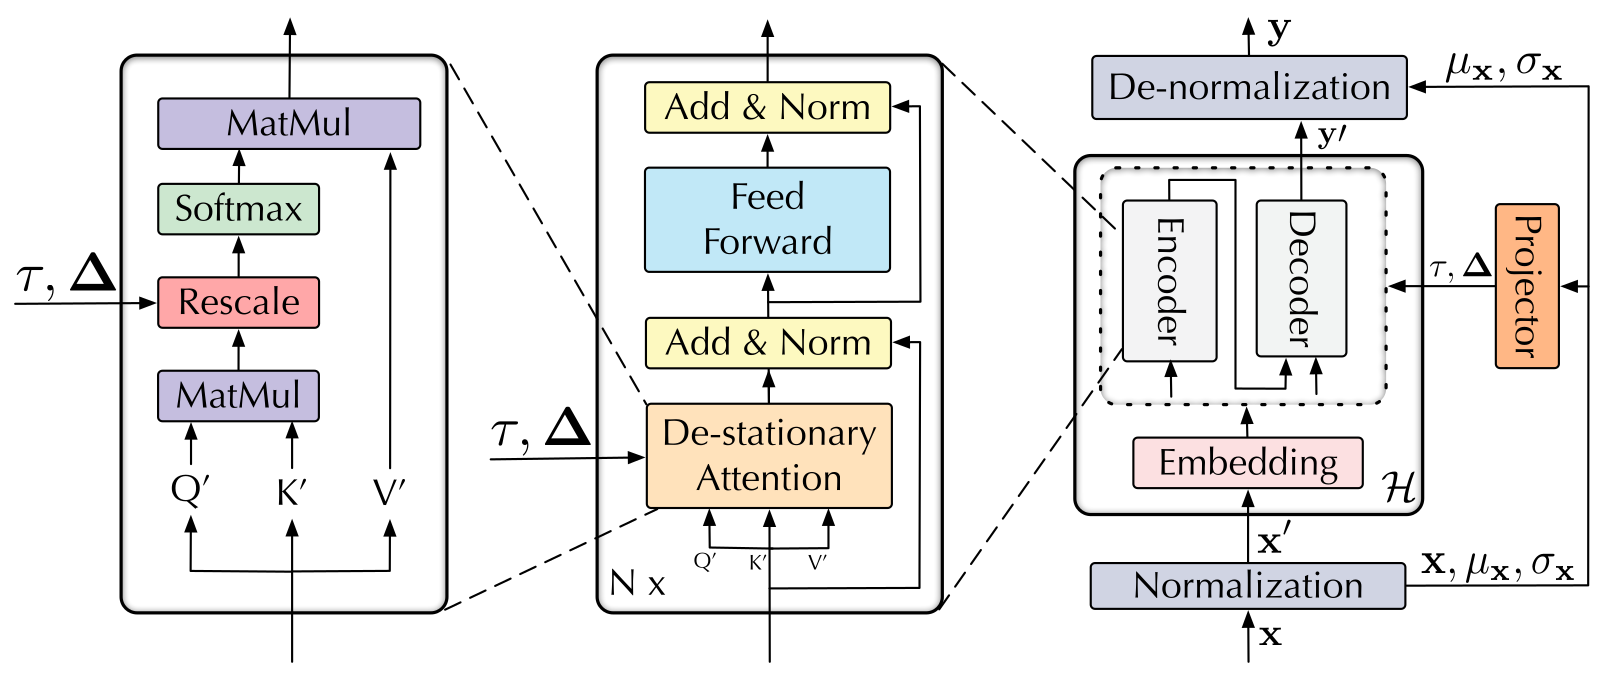
\includegraphics[width=0.5\linewidth]{notes.assets/image-20241018002155665.png}
    \caption{Non-Stationary Transformer}
    \label{fig:enter-label}
\end{figure}

\begin{thebibliography}{9}

\bibitem{tsmixer}
Si-An Chen, Chun-Liang Li, Nate Yoder, Sercan O. Arik, and Tomas Pfister.
\newblock TSMixer: An All-MLP Architecture for Time Series Forecasting.
\newblock 2023.
\newblock \url{https://arxiv.org/abs/2303.06053}.

\bibitem{ltsflinear}
Ailing Zeng, Muxi Chen, Lei Zhang, and Qiang Xu.
\newblock Are Transformers Effective for Time Series Forecasting?
\newblock 2022.
\newblock \url{https://arxiv.org/abs/2205.13504}.

\bibitem{tcnpaper}
Colin Lea, Michael D. Flynn, Rene Vidal, Austin Reiter, and Gregory D. Hager.
\newblock Temporal Convolutional Networks for Action Segmentation and Detection.
\newblock 2016.
\newblock \url{https://arxiv.org/abs/1611.05267}.

\bibitem{deepar}
David Salinas, Valentin Flunkert, and Jan Gasthaus.
\newblock DeepAR: Probabilistic Forecasting with Autoregressive Recurrent Networks.
\newblock 2019.
\newblock \url{https://arxiv.org/abs/1704.04110}.

\bibitem{inception}
Ismail Fawaz, Hassan, Benjamin Lucas, Germain Forestier, Charlotte Pelletier, Daniel F. Schmidt, Jonathan Weber, Geoffrey I. Webb, Lhassane Idoumghar, Pierre-Alain Muller, and François Petitjean.
\newblock InceptionTime: Finding AlexNet for time series classification.
\newblock \emph{Data Mining and Knowledge Discovery}, 34(6):1936–1962, sep 2020.
\newblock ISSN 1573-756X.
\newblock \url{http://dx.doi.org/10.1007/s10618-020-00710-y}.

\bibitem{wavenet}
Aaron van den Oord, Sander Dieleman, Heiga Zen, Karen Simonyan, Oriol Vinyals, Alex Graves, Nal Kalchbrenner, Andrew Senior, and Koray Kavukcuoglu.
\newblock WaveNet: A Generative Model for Raw Audio.
\newblock 2016.
\newblock \url{https://arxiv.org/abs/1609.03499}.

\bibitem{moderntcn}
Luo donghao and wang xue.
\newblock Modern{TCN}: A Modern Pure Convolution Structure for General Time Series Analysis.
\newblock In \emph{The Twelfth International Conference on Learning Representations}, 2024.
\newblock \url{https://openreview.net/forum?id=vpJMJerXHU}.

\bibitem{informer}
Haoyi Zhou, Shanghang Zhang, Jieqi Peng, Shuai Zhang, Jianxin Li, Hui Xiong, and Wancai Zhang.
\newblock Informer: Beyond Efficient Transformer for Long Sequence Time-Series Forecasting.
\newblock 2021.
\newblock \url{https://arxiv.org/abs/2012.07436}.

\bibitem{nst}
Yong Liu, Haixu Wu, Jianmin Wang, and Mingsheng Long.
\newblock Non-stationary Transformers: Exploring the Stationarity in Time Series Forecasting.
\newblock 2023.
\newblock \url{https://arxiv.org/abs/2205.14415}.

\bibitem{ssm}
Albert Gu, Karan Goel, and Christopher Ré.
\newblock Efficiently modeling long sequences with structured state spaces.
\newblock arXiv preprint arXiv:2111.00396, 2022.
\newblock URL \url{https://arxiv.org/abs/2111.00396}.

\bibitem{timesnet}
Haixu Wu, Tengge Hu, Yong Liu, Hang Zhou, Jianmin Wang, and Mingsheng Long.
\newblock TimesNet: Temporal 2D-variation modeling for general time series analysis.
\newblock arXiv preprint arXiv:2210.02186, 2023.
\newblock URL \url{https://arxiv.org/abs/2210.02186}.

\bibitem{autoformer}
Haixu Wu, Jiehui Xu, Jianmin Wang, and Mingsheng Long.
\newblock Autoformer: Decomposition transformers with auto-correlation for long-term series forecasting.
\newblock arXiv preprint arXiv:2106.13008, 2022.
\newblock URL \url{https://arxiv.org/abs/2106.13008}.

\bibitem{revin}
Taesung Kim, Jinhee Kim, Yunwon Tae, Cheonbok Park, Jang-Ho Choi, and Jaegul Choo.
\newblock Reversible instance normalization for accurate time-series forecasting against distribution shift.
\newblock In \emph{International Conference on Learning Representations}, 2022.
\newblock URL \url{https://openreview.net/forum?id=cGDAkQo1C0p}.


\end{thebibliography}


\end{document} 